\section*{Appendix}
\addcontentsline{toc}{section}{Appendix}
\renewcommand{\thesubsection}{\Alph{subsection}}
\setcounter{subsection}{0}

% Proof source: https://archive.cnx.org/contents/48100338-6af8-4c8b-afed-e15fd821cae6@5/discrete-time-markov-chains-state-classifications

\subsection{Proof of null recurrent chain}
\label{sec:proof-null-recurrent}

\begin{figure}[!b]
	\centering
	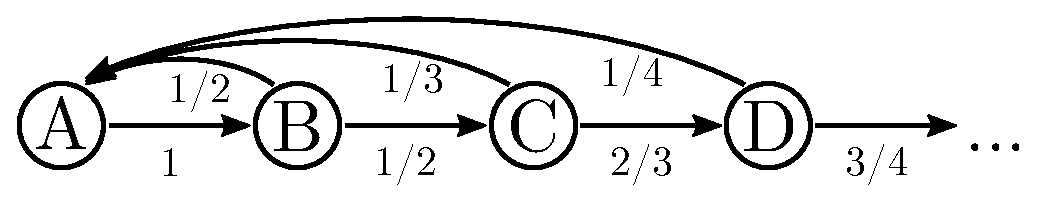
\includegraphics[width=0.6\textwidth]{appendix/mcmc-null-recurrent}
	\caption[Null recurrent Markov chain]{An example for a null recurrent Markov chain. It was introduced in figure \ref{fig:recurrent} as an example of a null recurrent Markov chain.}
	\label{fig:null-recurrent}
\end{figure}

In section \ref{sec:markov-properties} several properties of a Markov chain were introduced. An example of a \emph{null recurrent} Markov chain was given in figure \ref{fig:recurrent}. The null recurrent property of that chain will be proven in this appendix section. As a reminder the chain is shown again in figure \ref{fig:null-recurrent}. Also remind the definition of the random variable $T_{x_i}$ in equation \eqref{eq:first-comeback}, which is the number of steps necessary to come back to state $x_i$ for the \emph{first time}. A state is recurrent if $\Pb(T_{x_i} < \infty) = 1$, which corresponds to equation \eqref{eq:recurrent} and null recurrent if $\E[T_i] = \infty$, which was defined in \eqref{eq:first-comeback-expect} and the following.

First, a homogen Markov chain is assumed and an infinite state space $S = \{x_1, x_2, x_3, x_4, ...\} = \{A, B, C, D, ...\}$ is given. $\Pb(T_{x_i} = t)$ will be denoted by $q_{x_i}^t$. It is the probability to come back to state $x_i$ for the first time after $t$ steps. Therefore, starting from state $A$, the probability to come back to state $A$ in only one step is

\begin{equation}
q_A^1 = \Pb(T_A = 1) = \Pb(X_1 = A | X_0 = A) = p_{AA} = 0.
\end{equation}

Since $A$ has no self-loop, it is impossible to come back to $A$ in just one step. For two steps, a non-zero probability exists:

\begin{equation}
\begin{split}
q_A^2 &= \Pb(T_A = 2)\\
&= \Pb(X_1 = B | X_0 = A) \cdot \Pb(X_2 = A | X_1 = B)\\
&= p_{AB} \cdot p_{BA} = 1 \cdot \frac{1}{2} = \frac{1}{2}
\end{split}
\end{equation}

Results are similar for $t=3$, $t=4$ and $t=5$ steps:

\begin{subequations}
\begin{equation}
q_A^3 = p_{AB} \cdot p_{BC} \cdot p_{CA} = 1 \cdot \frac{1}{2} \cdot \frac{1}{3} = \frac{1}{6}
\end{equation}
\begin{equation}
q_A^4 = p_{AB} \cdot p_{BC} \cdot p_{CD} \cdot p_{DA} = 1 \cdot \frac{1}{\cancel{2}} \cdot \frac{\cancel{2}}{3} \cdot \frac{1}{4} = \frac{1}{3} \cdot \frac{1}{4} = \frac{1}{12}
\end{equation}
\begin{equation}
q_A^5 = p_{AB} \cdot p_{BC} \cdot p_{CD} \cdot p_{DE} \cdot p_{EA} = 1 \cdot \frac{1}{\cancel{2}} \cdot \frac{\cancel{2}}{\cancel{3}} \cdot \frac{\cancel{3}}{4} \cdot \frac{1}{5} = \frac{1}{4} \cdot \frac{1}{5} = \frac{1}{20}
\end{equation}
\end{subequations}

It can easily be seen that $q_A^t$ follows a specific rule, namely

\begin{equation}
q_A^t = \frac{1}{t-1} \frac{1}{t},
\end{equation}

for all $t>1$. Note that it does not hold for $t=1$.

Using this rule, the probability to come back to state $A$ can be obtained by

\begin{equation}
\begin{split}
\Pb(T_A < \infty) &= \sum_{t=1}^\infty \Pb(T_A = t) = \sum_{t=1}^\infty q_A^t\\
&= 0 + \sum_{t=2}^\infty \frac{1}{t-1} \frac{1}{t} = \sum_{t=1}^\infty \frac{1}{t} \frac{1}{t+1}.
\end{split}
\end{equation}

With induction it can be shown that

\begin{equation}
\Pb(T_A < \infty) = \sum_{t=1}^\infty \frac{1}{t} \frac{1}{t+1} = \lim_{n \to\infty} \frac{n-1}{n} = 1.
\end{equation}

Hence, equation \eqref{eq:recurrent} is fulfilled and state $A$ is recurrent. It remains to show that the state is also null recurrent. In order to verify this, the expectation value can be calculated using

\begin{equation}
\begin{split}
\E[T_A] &= \sum_{t=1}^\infty t \cdot \Pb(T_A = t)\\
&= 0 + \sum_{t=2}^\infty t \cdot \frac{1}{t-1} \frac{1}{t} = \sum_{t=2}^\infty \frac{1}{t-1} = \sum_{t=1}^\infty \frac{1}{t} = \infty,
\end{split}
\end{equation}

where the last step follows from the harmonic series. It was possible to show that the expected number of steps, necessary to come back to state $A$ for the first time, are infinite. Equation \eqref{eq:first-comeback-expect} is fulfilled and state $A$ is null recurrent.

\hfill$\square$

\newpage

\subsection{Testing phase with STDP}
\label{sec:appendix:stdp}

\begin{figure}[!b]
    \centering
    \begin{subfigure}{0.48\textwidth}
    	\centering
        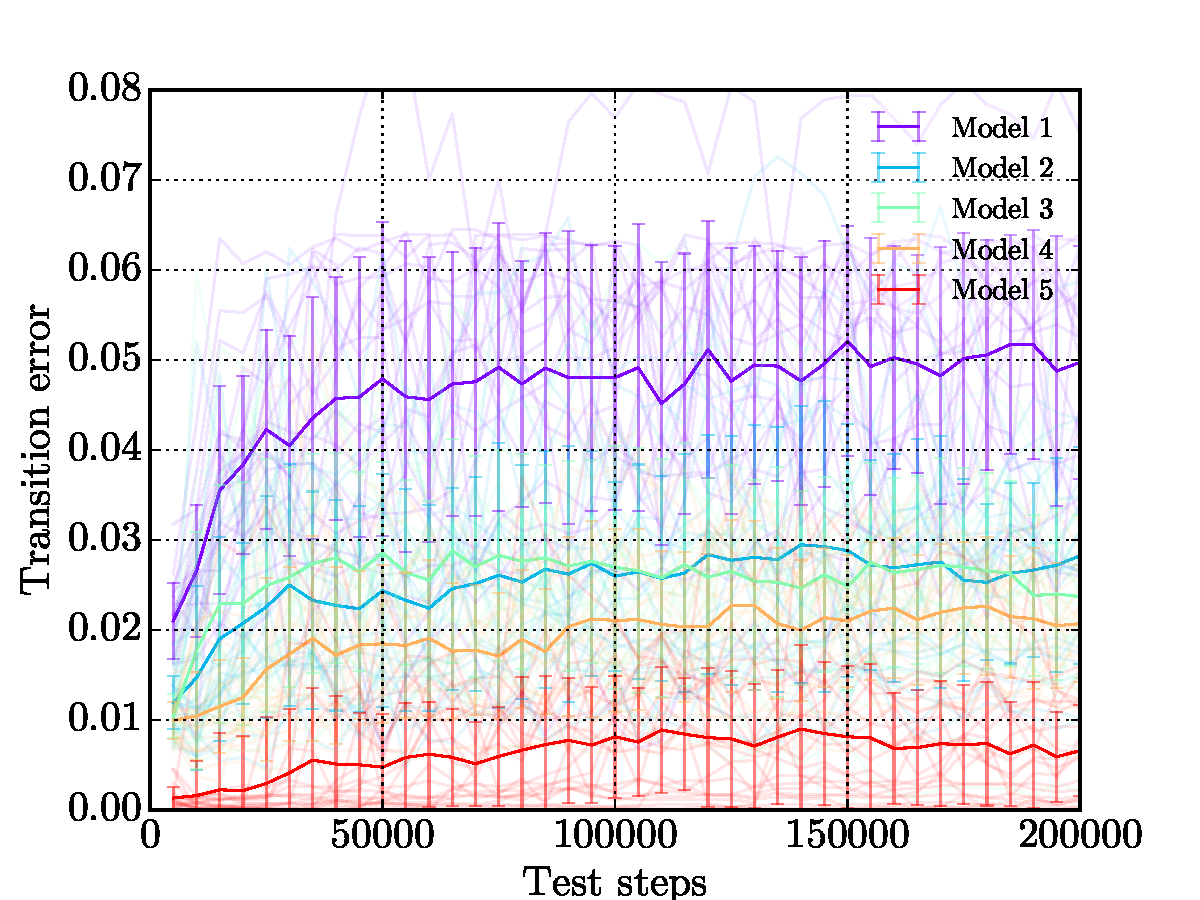
\includegraphics[width=\textwidth]{appendix/stdp_with_test_traces_distances}
        \caption{}
        \label{fig:stdp-with-trace}
    \end{subfigure}
    \hfill
    \begin{subfigure}{0.48\textwidth}
    	\centering
        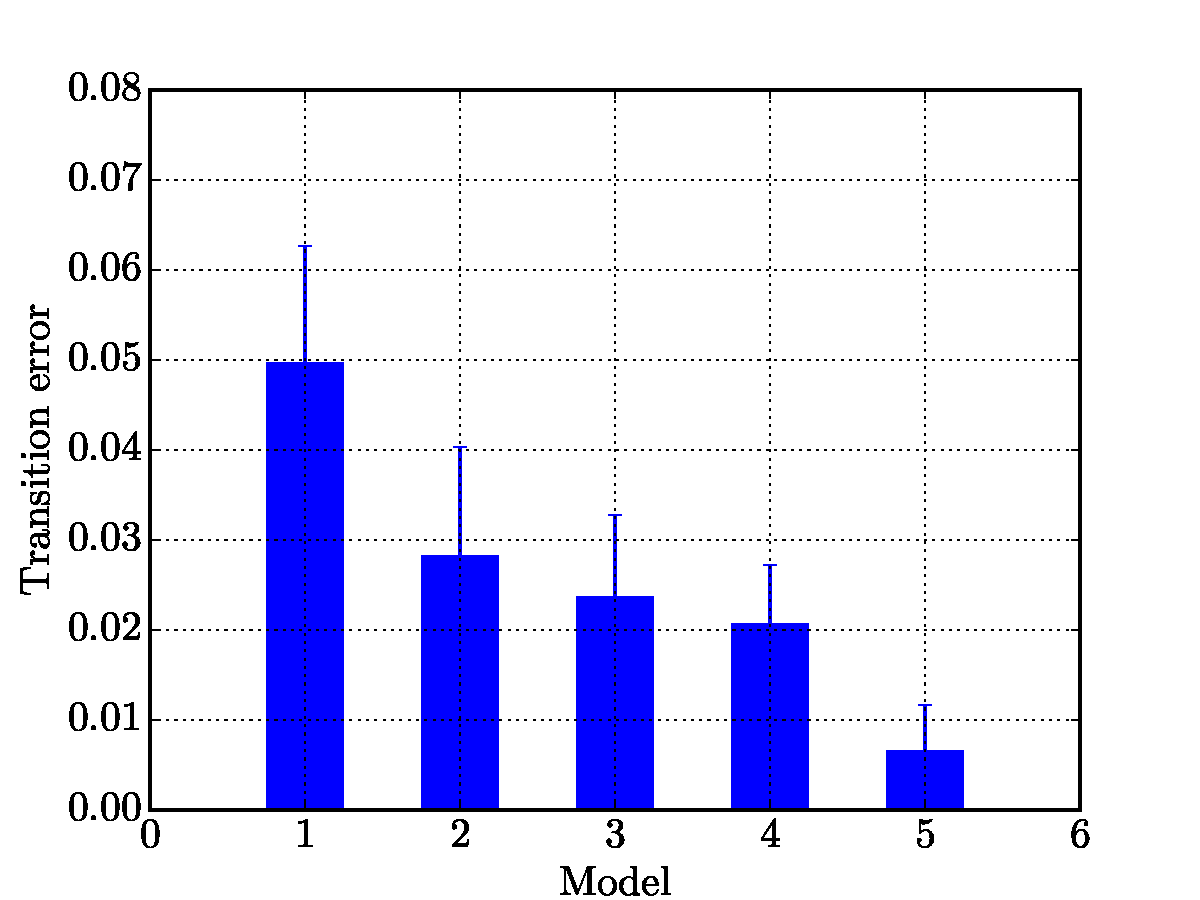
\includegraphics[width=\textwidth]{appendix/stdp_with_performance_distances}
        \caption{}
        \label{fig:stdp-with-perf}
    \end{subfigure}
    \begin{subfigure}{0.48\textwidth}
    	\centering
        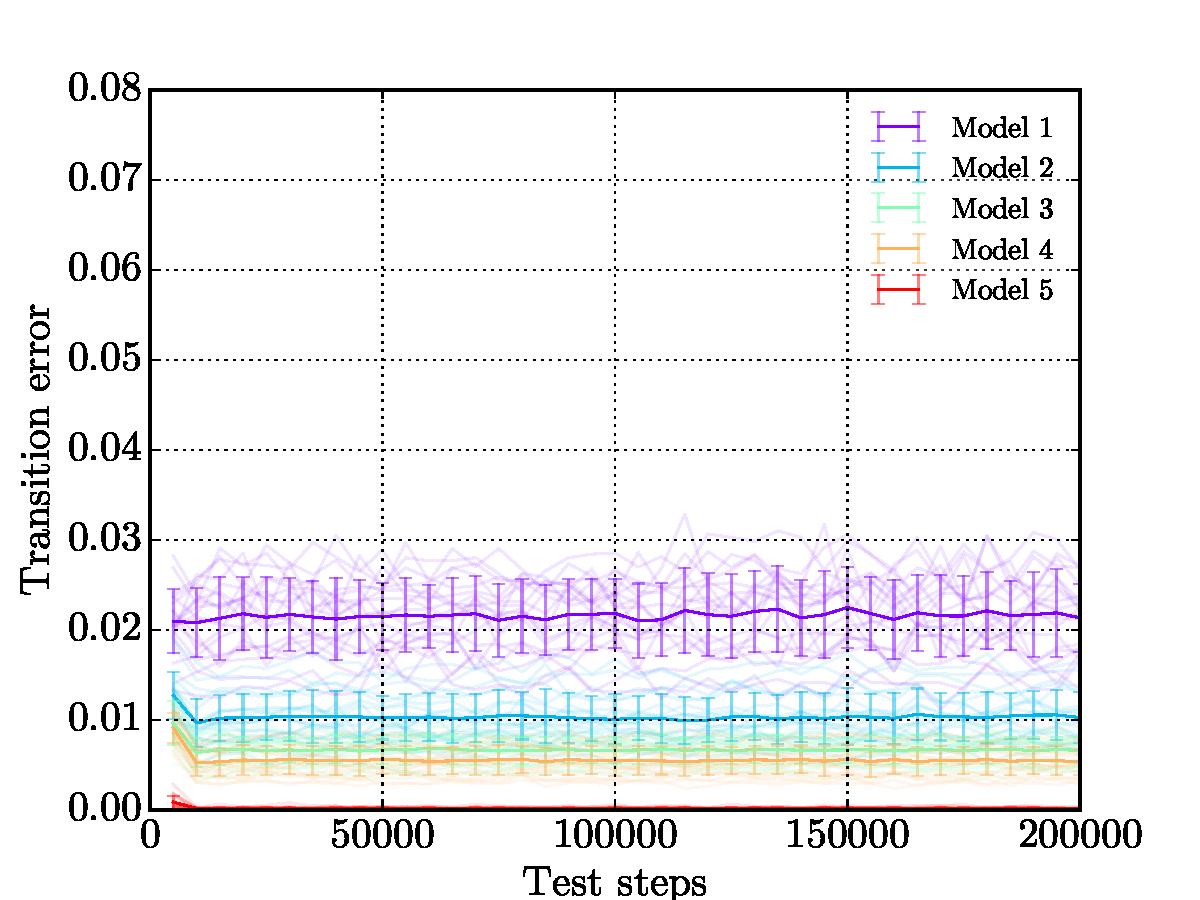
\includegraphics[width=\textwidth]{appendix/stdp_without_test_traces_distances}
        \caption{}
        \label{fig:stdp-without-test}
    \end{subfigure}
    \hfill
    \begin{subfigure}{0.48\textwidth}
    	\centering
        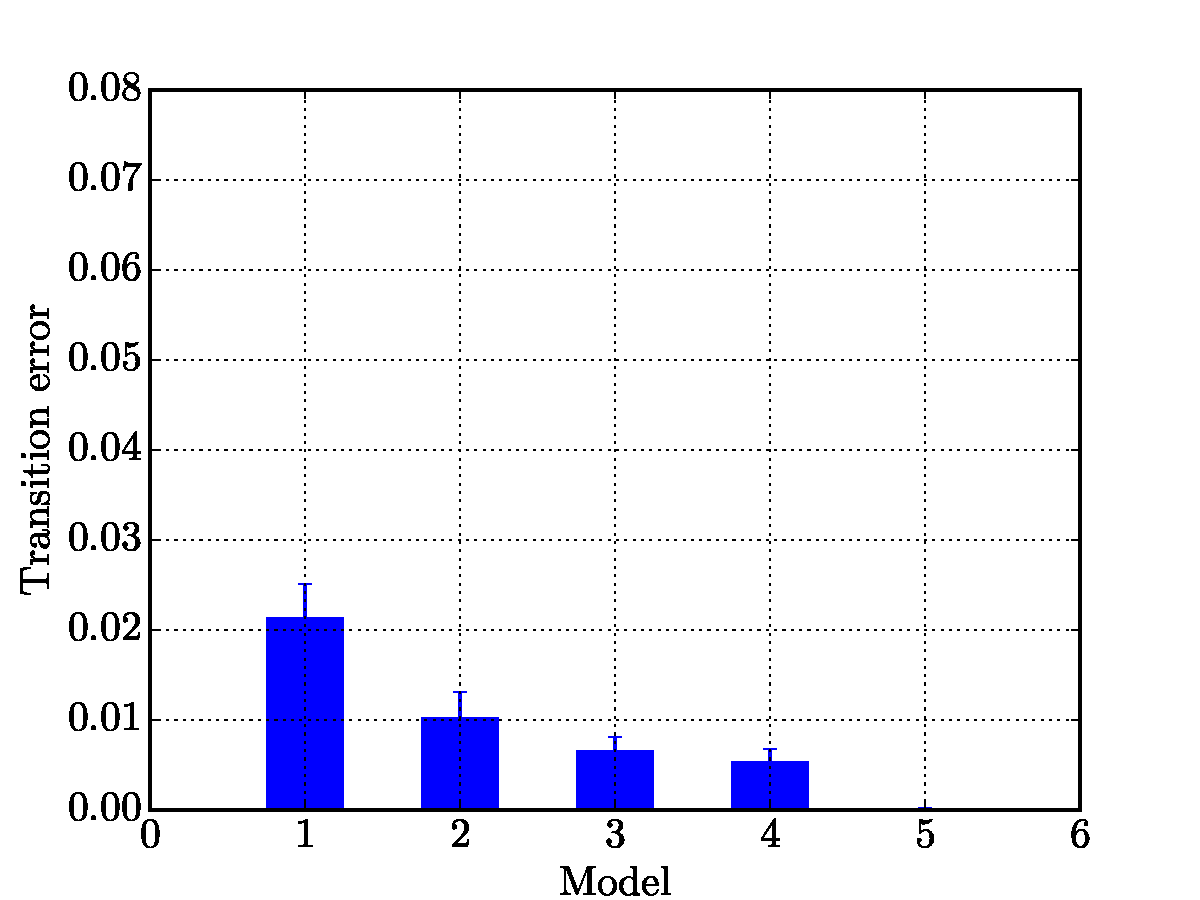
\includegraphics[width=\textwidth]{appendix/stdp_without_performance_distances}
        \caption{}
        \label{fig:stdp-without-perf}
    \end{subfigure}
    \caption[Performance with and without STDP in testing phase]{Performance with and without \acs{stdp} in testing phase. \textbf{a)} shows that the error increases quite fast in the testing phase with \acs{stdp}, compared to \textbf{c)}, where \acs{stdp} was switched off. \textbf{b)} and \textbf{d)} shows the performance at the end of the testing phase for both cases. As the error and the standard error is higher in the case with \acs{stdp}, the differences between the models are mainly maintained. Note that the testing phase was extended to $T_\test = 200,000$ steps and that the $y$-axis of the plots is fixed to $0.08$ for comparison. Error bars indicate standard errors.}
    \label{fig:stdp-with-without}
\end{figure}

The \acf{stdp} is responsible for the dynamics in the weights. It was applied while training to adjust the weights with respect to the time-dependent input patterns. Afterwards, while no-plastic training and while testing, \acs{stdp} was switched off in order to sustain the learned structure. In results, e.g. in figure \ref{fig:mc1-test_traces-transition}, it was shown that the static structure in the testing phase results in a constant performance. If \acs{stdp} is active in testing phase and, therefore, weights are further adapted, spontaneous activity should lead to random changes in the weights, which will increasingly occur independent from the initial Markov chain transitions. Subsequently, the stored state transitions should decay. The testing phase was extended to $T_\test = 200,000$ steps to be able to observe the process for a longer time and the model series II from figure \ref{fig:mc2-models} was used with $5$ models. 

Figure \ref{fig:stdp-with-trace} shows that the network `forgets' the stored information and the effect seems to be stronger for those Markov models, where errors were initially higher. The results can be compared to figure \ref{fig:stdp-without-test}, where also $T_\test = 200,000$ were simulated, but with \acs{stdp} switched off, as it was done in all previous simulations. The error increases quickly in the beginning and seems to maintain at a specific level. Interestingly, the differences between the models remain over the whole $200,000$ steps. Finally, figures \ref{fig:stdp-with-perf} and \ref{fig:stdp-without-perf} show the performance for both cases at the end of the testing phase. Those plots support the prior analysis. As the error and the standard error is higher in the simulation with \acs{stdp}, compared to the simulation without it, the differences between the models are basically maintained.

\newpage

\subsection{No-plastic training}
\label{sec:appendix:noplastic}

The length of the no-plastic training phase, which was introduced in section \ref{sec:train}, should have no influence on the performance. Its objective is to classify the current state of the network, when only spontaneous activity is in the network. Even if the input is still active in the no-plastic training phase, the main training effect should come from the plastic training phase, when the network adjusts the weights using \acs{stdp} and input is given for a long time of $T_\plastic = 50,000$ steps in most cases.

The number of steps in the no-plastic training phase $T_\noplastic$ was varied for model series II from figure \ref{fig:mc2-models} with $5$ models. As can be seen in figure \ref{fig:noplastic}, there is no influence on the performance of the models. The performance is independent from the number of no-plastic training steps. There are some slight differences in model $1$, but they are not significant ($p > 0.05$). Note that it is not possible to set the number of training steps below the number of steps to compare with. That actually means that necessarily $T_\noplastic > \tilde{T}_{\text{compare}}$, as already discussed in the methods section.

\begin{figure}[!b]
	\centering
	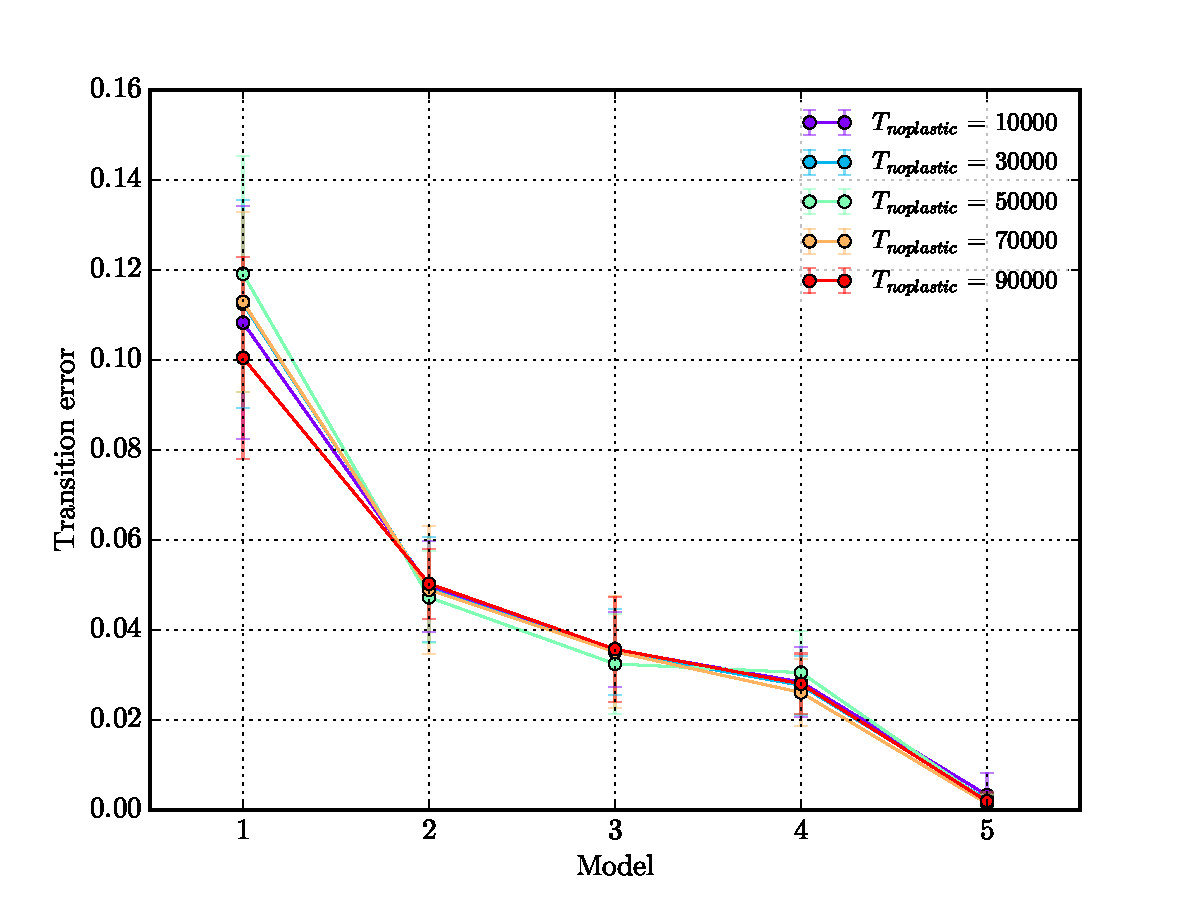
\includegraphics[width=0.85\textwidth]{appendix/noplastic_train}
	\caption[Influence of the length of the no-plastic training phase]{Influence of the length of the no-plastic training phase $T_\noplastic$. The parameter was chosen between $T_\noplastic = 10,000$ and $T_\noplastic = 90,000$. The length of the no-plastic training phase does not influence the performance of the models.}
	\label{fig:noplastic}
\end{figure}

\clearpage

\subsection{Hamming classification}
\label{sec:appendix:hamming}

\begin{figure}[p]
    \centering
    \begin{subfigure}{0.48\textwidth}
    	\centering
        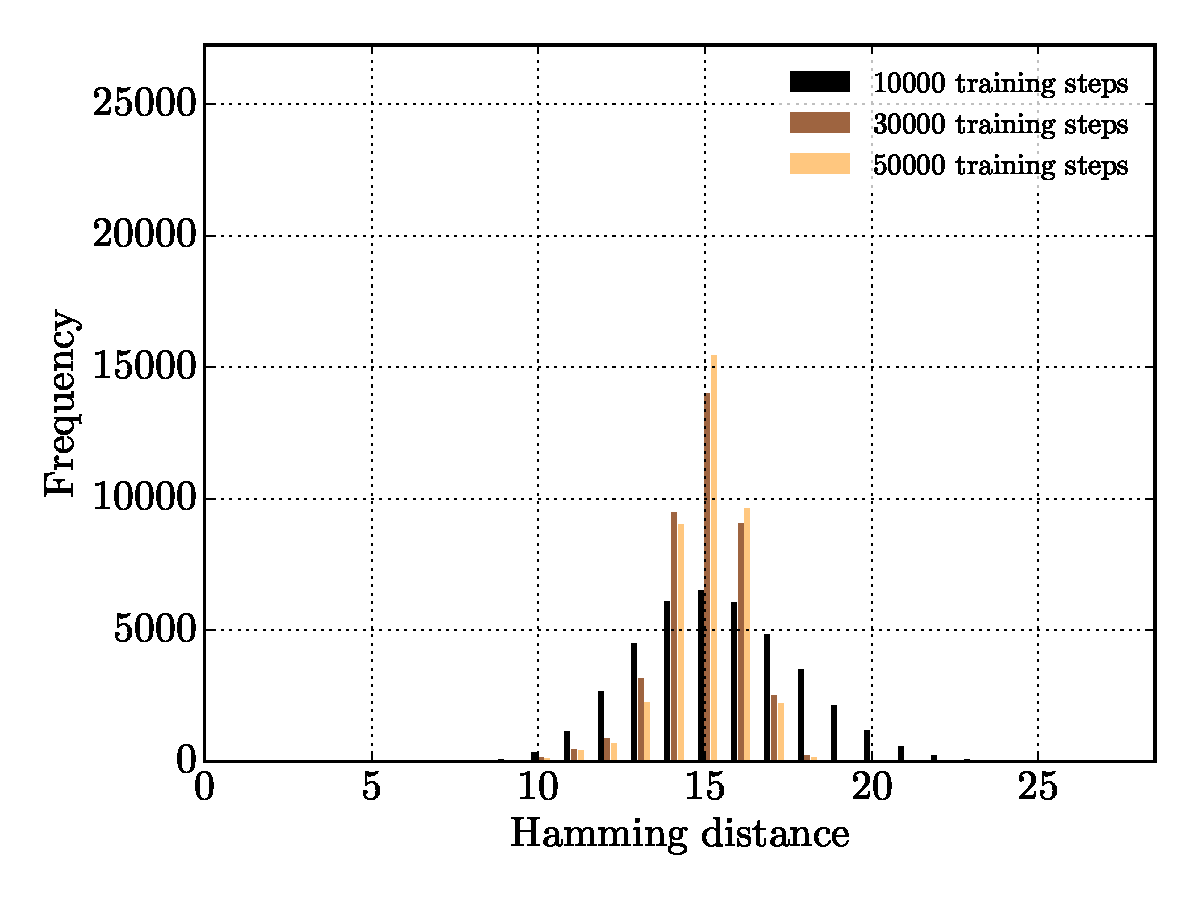
\includegraphics[width=\textwidth]{appendix/hamming_freqs_model1}
        \caption{Model $1$}
        \label{fig:ham-freq-1}
    \end{subfigure}
    \hfill
    \begin{subfigure}{0.48\textwidth}
    	\centering
        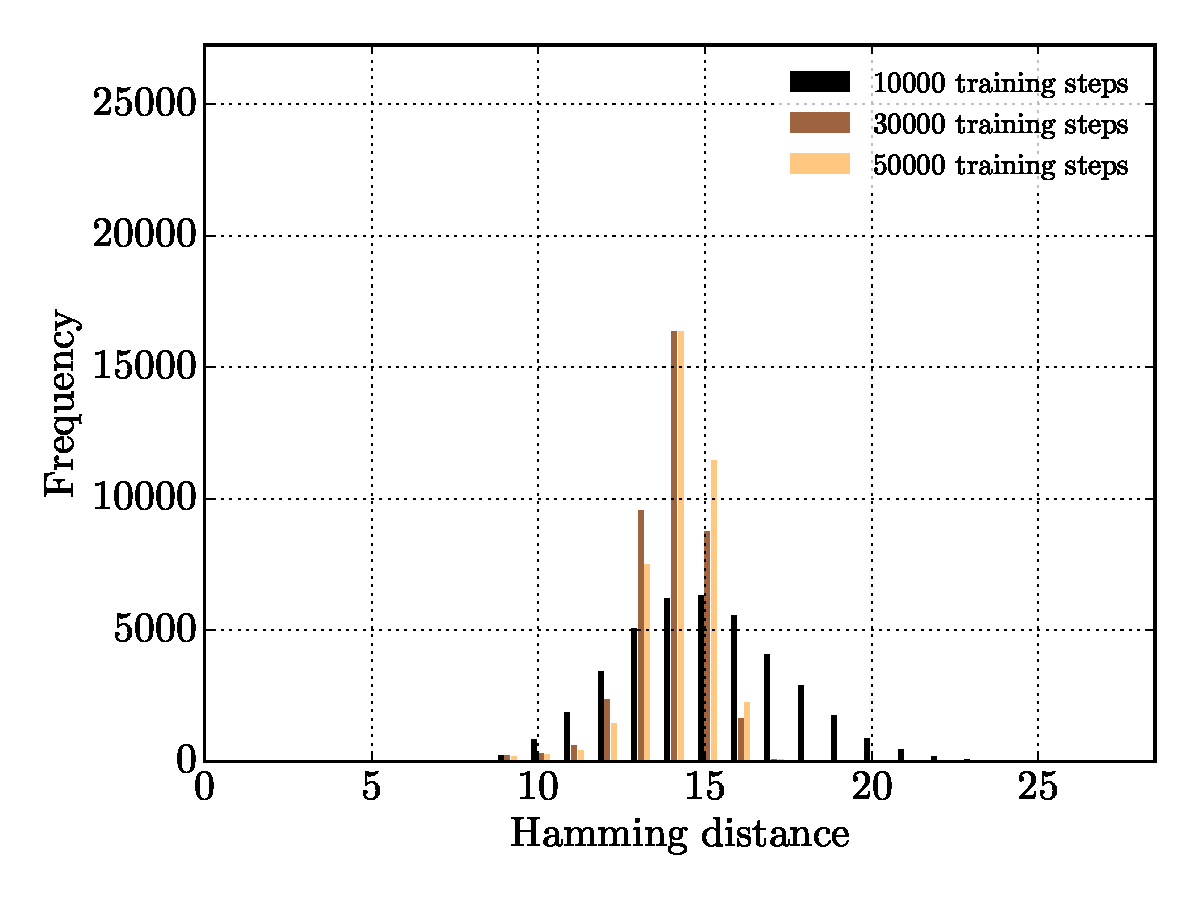
\includegraphics[width=\textwidth]{appendix/hamming_freqs_model2}
        \caption{Model $2$}
        \label{fig:ham-freq-2}
    \end{subfigure}
    \begin{subfigure}{0.48\textwidth}
    	\centering
        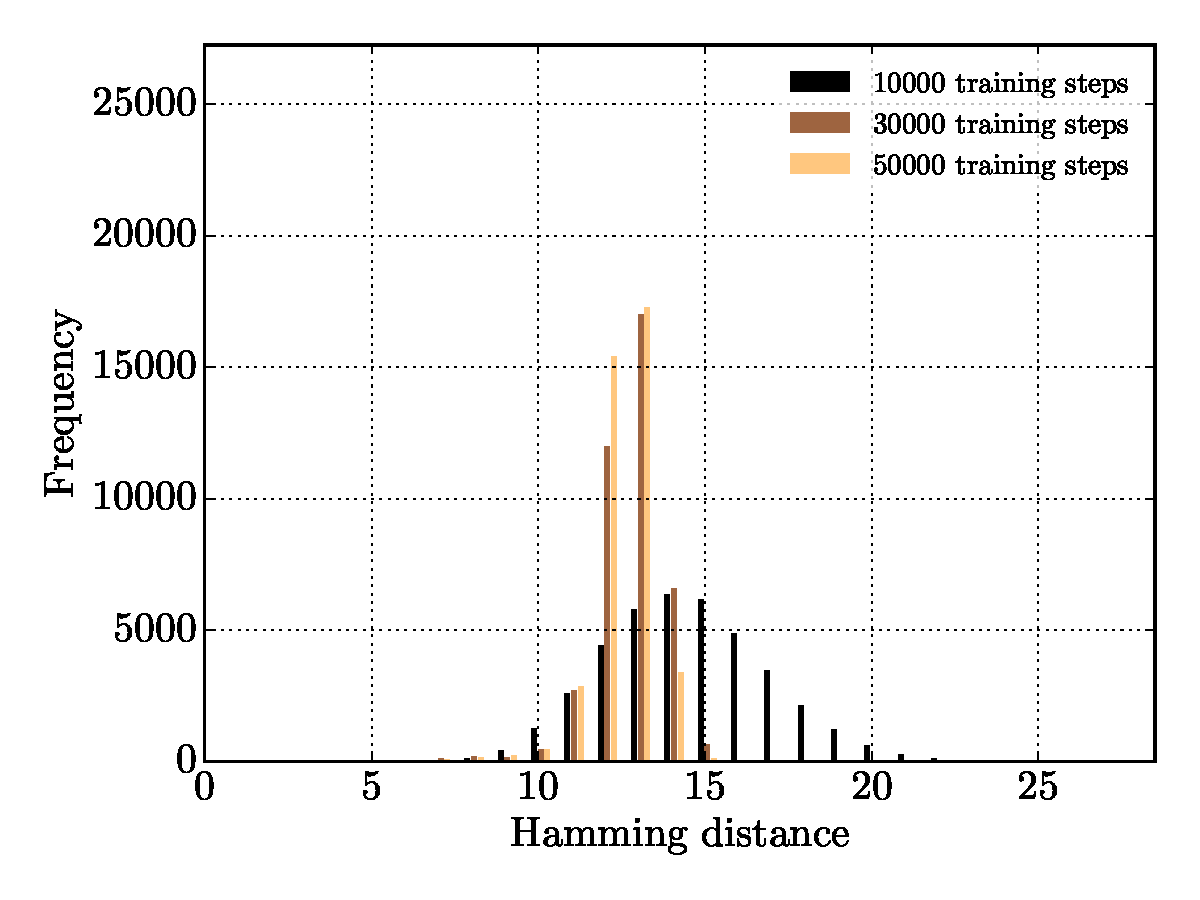
\includegraphics[width=\textwidth]{appendix/hamming_freqs_model3}
        \caption{Model $3$}
        \label{fig:ham-freq-3}
    \end{subfigure}
    \hfill
    \begin{subfigure}{0.48\textwidth}
    	\centering
        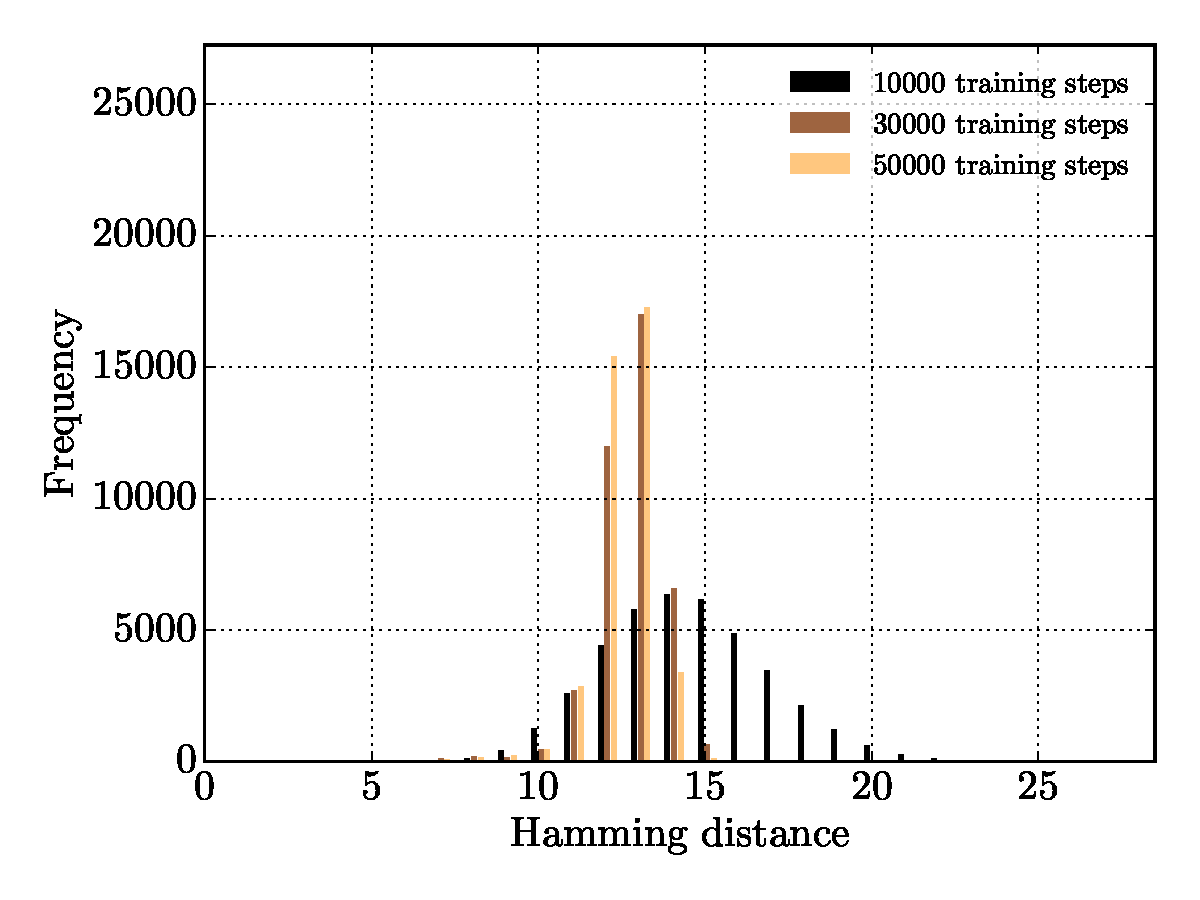
\includegraphics[width=\textwidth]{appendix/hamming_freqs_model3}
        \caption{Model $4$}
        \label{fig:ham-freq-4}
    \end{subfigure}
    \begin{subfigure}{0.48\textwidth}
    	\centering
        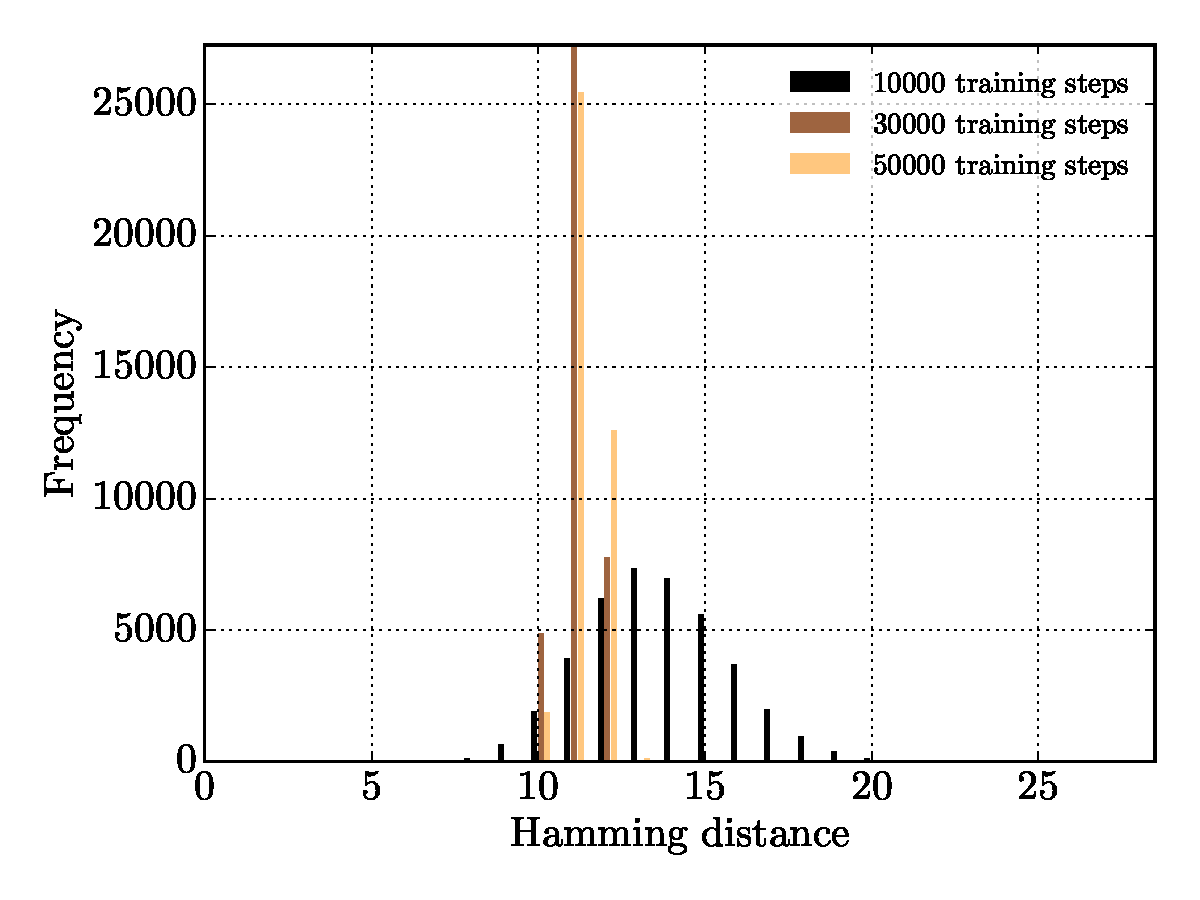
\includegraphics[width=\textwidth]{appendix/hamming_freqs_model5}
        \caption{Model $5$}
        \label{fig:ham-freq-5}
    \end{subfigure}
    \caption[Histograms of minimum hamming distances for 5 models]{Histograms of minimum hamming distances for 5 models. The minimum hamming distances are normally distributed. The variances of the minimum hamming distances decrease if training is increased. The mean also decreases, as long as state $A$ is not to unlikely. Furthermore, the mean decreases if state $A$ is more and more equally connected to the other states and the states in the model becomes more regular.}
    \label{fig:ham-freqs}
\end{figure}

The purpose of this section is to evaluate the classification mechanism, based on the hamming distance. The systematic model series II was used for evaluation,, shown in figure \ref{fig:mc2-models} in results. The series was realized with $5$ models. The hamming distance calculation was introduced in section \ref{sec:state-classification}. In a first step, histograms were plotted, showing the frequencies of the smallest hamming distances for every step in the testing phase, where any testing phase step was compared with all comparison steps from the no-plastic testing phase. Results are shown in figure \ref{fig:ham-freqs}. There are three notable effects:

\begin{figure}[!t]
    \centering
    \begin{subfigure}{0.48\textwidth}
    	\centering
        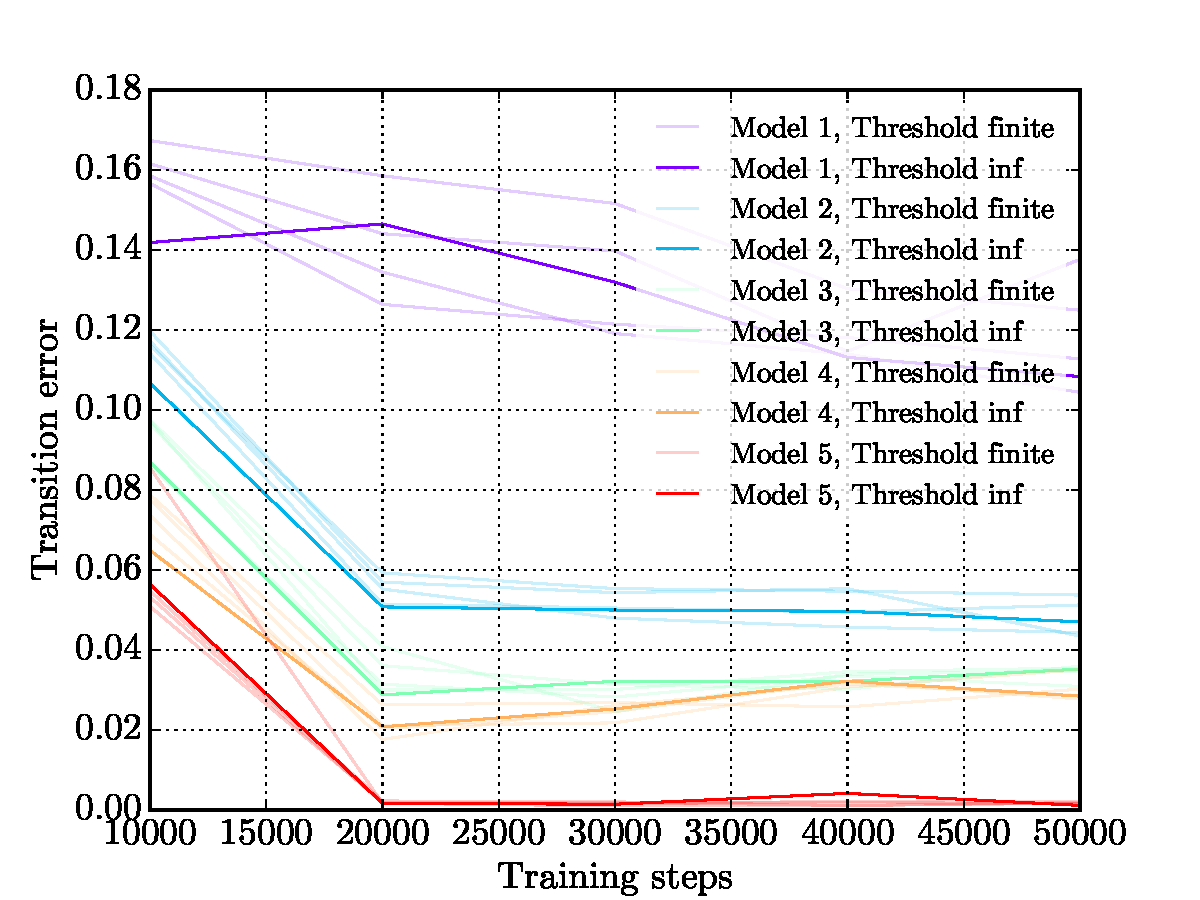
\includegraphics[width=\textwidth]{appendix/hamming_distances_training_steps_with_thresholds}
        \caption{}
        \label{fig:ham-thesholds}
    \end{subfigure}
    \hfill
    \begin{subfigure}{0.48\textwidth}
    	\centering
        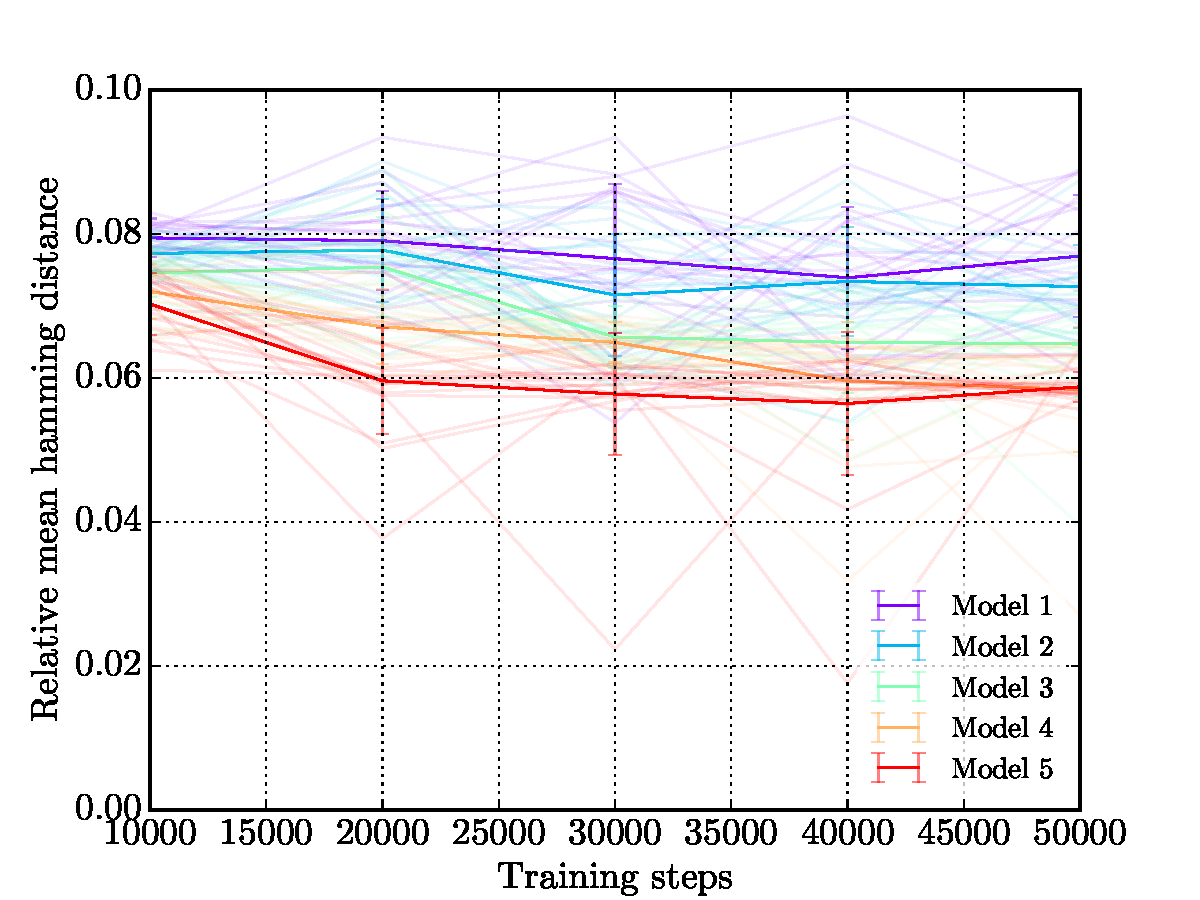
\includegraphics[width=\textwidth]{appendix/hamming_distances_training_steps_hamming}
        \caption{}
        \label{fig:ham-training-hamming}
    \end{subfigure}
    \caption[Performance results associated with hamming distances]{Performance results associated with hamming distances. In \textbf{a)} thresholds of $20,22,24$ and $26$ were applied. If the minimum hamming distance exceeded that threshold, the current pattern was classified as `unknown'. In the legend they are represented with the transparent lines for each model. They are compared to the default case, were no threshold was applied. In that case the threshold is infinity. It is represented by the opaque line for each model. In figure \textbf{b)}, the mean minimum hamming distance was calculated and divided by the maximum possible hamming distance $N^E$. The relative mean hamming distance can be used as a performance measure. Differences between the models are present and a training effect occurs. But since this measure is very robust and, therefore, effects are very small compared to the transition error, this performance measure was not used.}
    \label{fig:ham-thraining}
\end{figure}

\begin{itemize}
\item A Kolmogorov-Smirnov test was performed, showing that all minimum hamming distances are normally distributed ($p > 0.05$).
\item The more the model contains less probable states (model $1$ has fewest transition probability to state $A$, model $5$ is equal for every state), the higher is the mean of the minimum hamming distances in tendency.
\item The more the network was trained, the lower is the variance and the mean of the minimum hamming distances in tendency. This effect is stronger for models with states which occur with similar probabilities.
\end{itemize}

Furthermore, it was checked if the classification method has an influence on the performance. In section \ref{sec:state-classification} a parallel to the $k$-nearest neighbor algorithm with $k=1$ was drawn. The classification mechanism does only search for the one activity pattern which is closest. The hamming distance could be the same for activity patterns that belong to different Markov states. In that case, the algorithm just chooses the first one. It would be possible to apply a threshold which classifies states as `unknown' if the minimum hamming distance is too high. That is the case, if the state in the network is not very clear. It was checked if such a stricter rule, using a threshold, influences the behavior. Figure \ref{fig:ham-thesholds} shows that  this is not the case. The transparent lines show the performance of different thresholds. The opaque line represents a threshold of infinity, which equals no threshold at all, and therefore represents the algorithm which was used by default. If a threshold is applied, its performance seems to be very similar to the performance of the infinite threshold. Hence, the original algorithm seems to be very robust.

Finally, the relative mean hamming distance was calculated. The minimum hamming distances were averaged and divided by the maximum possible hamming distance $N^E$ in order to provide another performance measure. The better the model is learned, the lower should be the minimum hamming distance. Indeed, figure \ref{fig:ham-training-hamming} shows that the relative mean hamming distance behaves similar to the other performance measures. But the differences between the models and the decrease in performance, due to training, seems to be very low. Therefore, the relative mean hamming distance is not an appropriate performance measure. On the other hand, it shows again that the hamming distance is very robust between the models and regarding more or less training.

\newpage

\subsection{Models close to equal probabilities}
\label{sec:appendix:close}

In most cases, the `equal' model, where the probability of all available connections is $0.5$, was outstanding in performance. There was a drop between this model and the very next model, e.g. in figure \ref{fig:mc2-performance-distance}, \ref{fig:mc3-performance-distance} or \ref{fig:mc6-performance-distance} in the results section. In this section, starting from the `equal' model, the probabilities were varied in very small steps to be able to observe the behavior for very small changes. For evaluation, the model series II from figure \ref{fig:mc2-models} was adapted to a series which is shown in figure \ref{fig:mc2b-models}. This series was applied with $76$ steps between the left and right model. Therefore, the probabilities were changed in very small steps.

\begin{figure}[!h]
	\centering
	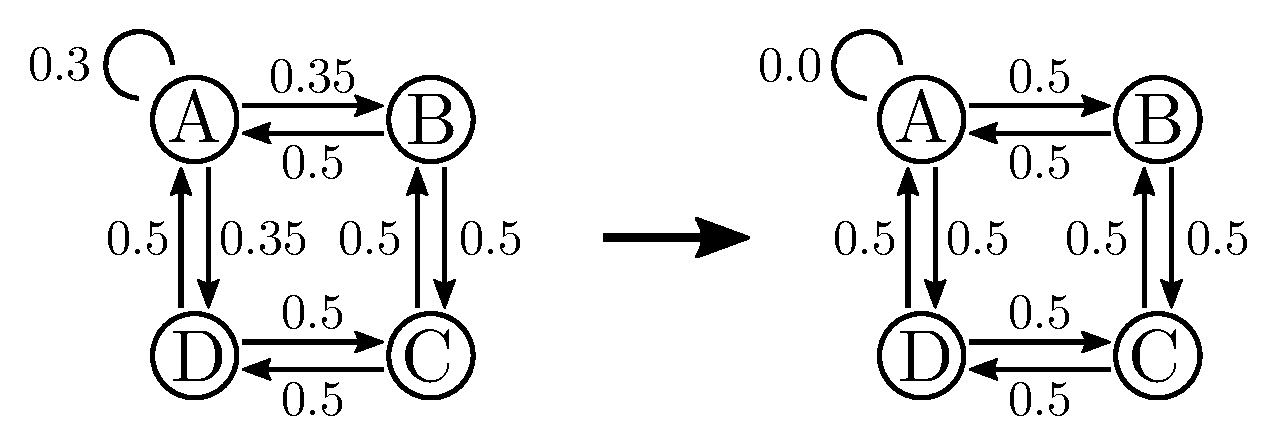
\includegraphics[width=0.85\textwidth]{appendix/mc2b_models}
	\caption[Model series close to equal probabilities]{Model series close to equal probabilities. This series is adapted from the model series II in figure \ref{fig:mc2-models}, where the starting probability is already chosen more close to the `equal' model. This series was divided into $76$ steps with very small probability changes.}
	\label{fig:mc2b-models}
\end{figure}

The results are shown in figure \ref{fig:mc2b-performance}. Starting from the right, were all probabilities are equal, the error starts to increase very fast. Small changes seem to influence the performance more strongly if the models are close to the `equal' model. The performance change of the models on the left side is small. Therefore, those models seem to be more robust to changes of the probabilities. Whereas the models on the right are very sensitive to changes of the probabilities.

\begin{figure}[p]
	\centering
	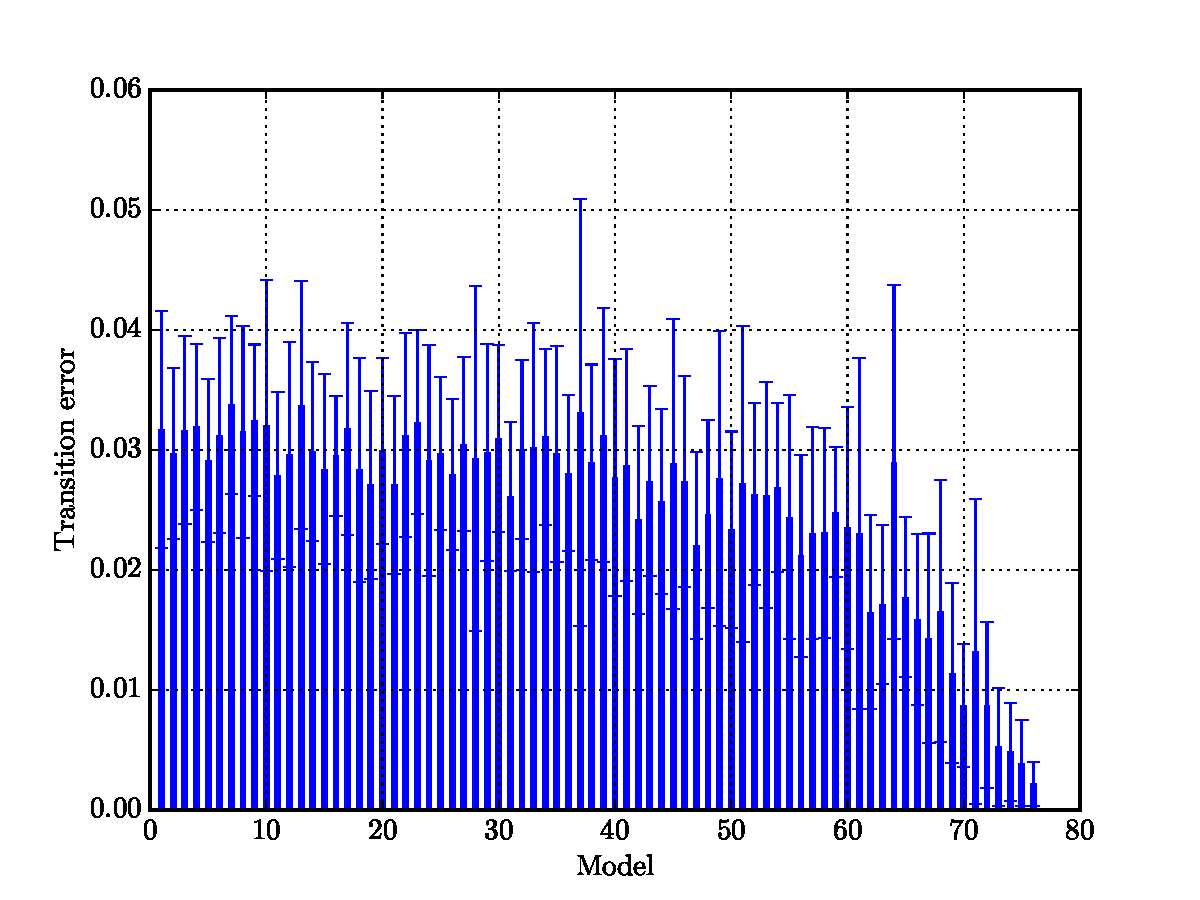
\includegraphics[width=0.85\textwidth]{appendix/mc2b_performance_distances}
	\caption[Performance of model series close to equal probabilities]{Performance of model series close to equal probabilities. $76$ models were applied and the probabilities were changed in very small steps. The network is sensitive to changes around the `equal' model (last model on the right) and becomes more robust towards the more unequal models (right to left).}
	\label{fig:mc2b-performance}
\end{figure}

\clearpage

\subsection{IP learning rate}
\label{sec:appendix:eta}

The \acs{ip} mechanism was suggested to explain the performance differences of the different input patterns, sampled from the Markov chains. The \acl{ip} rule is build with three parameters, introduced in equation \eqref{eq:hip-ind} in methods. $\bar H^\IP$ and $\sigma^\IP$ were already tested in section \ref{sec:ip-hyp} in results, but the impact of the learning rate parameter $\eta_\IP$ remains to be checked. The model series II from figure \ref{fig:mc2-models} was used and applied with $5$ models.

Figure \ref{fig:eta-small} shows that a very small $\eta_\IP = 0.0002$ increases the burn-in time in the testing phase. The network needs a long time until it finds a stable performance. If the parameter is very high, like in figure \ref{fig:eta-huge}, where $\eta_\IP = 0.002$, the performance starts to be stable after the first few steps in testing phase. This also happens for the default case with $\eta_\IP = 0.001$, shown in figure \ref{fig:eta-norm}.

\begin{figure}[!b]
    \centering
    \begin{subfigure}{0.48\textwidth}
    	\centering
        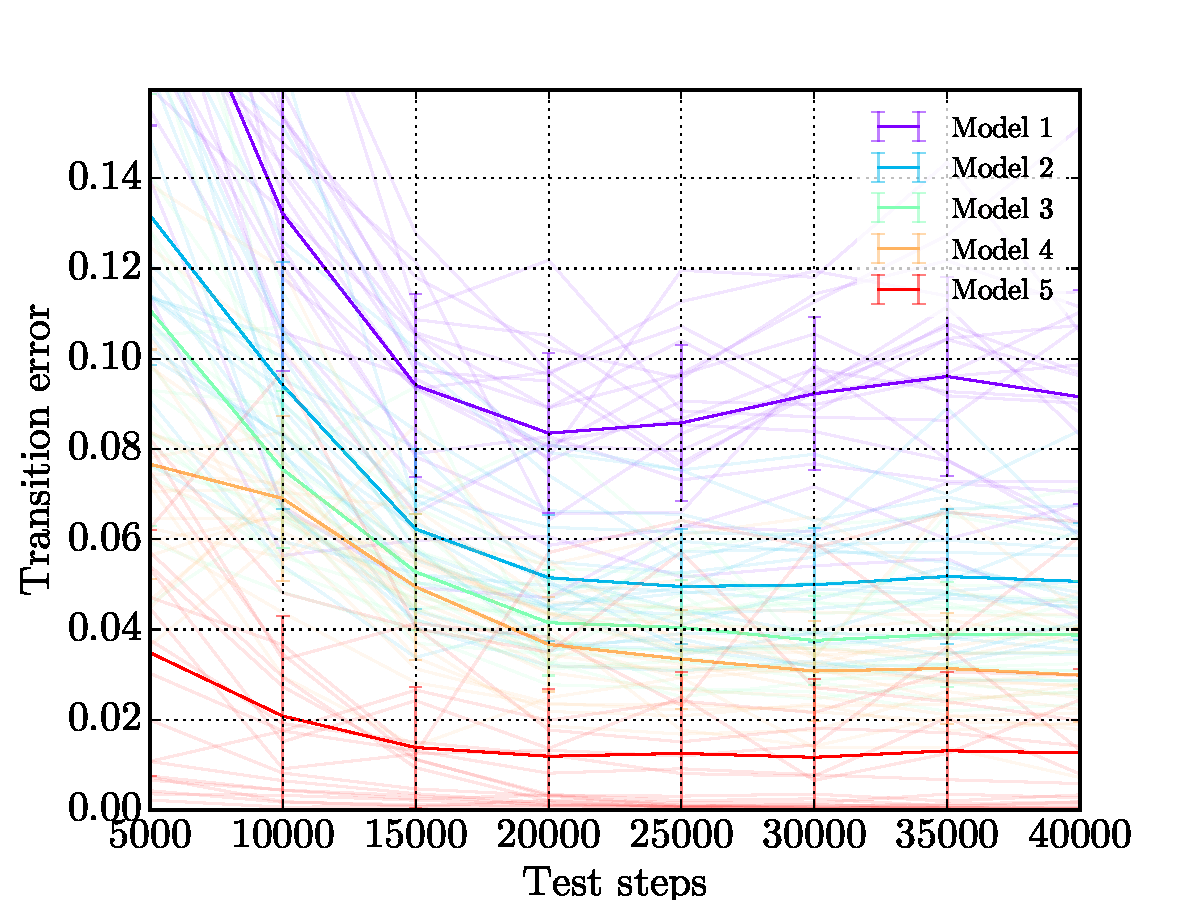
\includegraphics[width=\textwidth]{appendix/etaip_test_traces_distances_smallhip}
        \caption{$\eta_\IP = 0.0002$}
        \label{fig:eta-small}
    \end{subfigure}
    \hfill
    \begin{subfigure}{0.48\textwidth}
    	\centering
        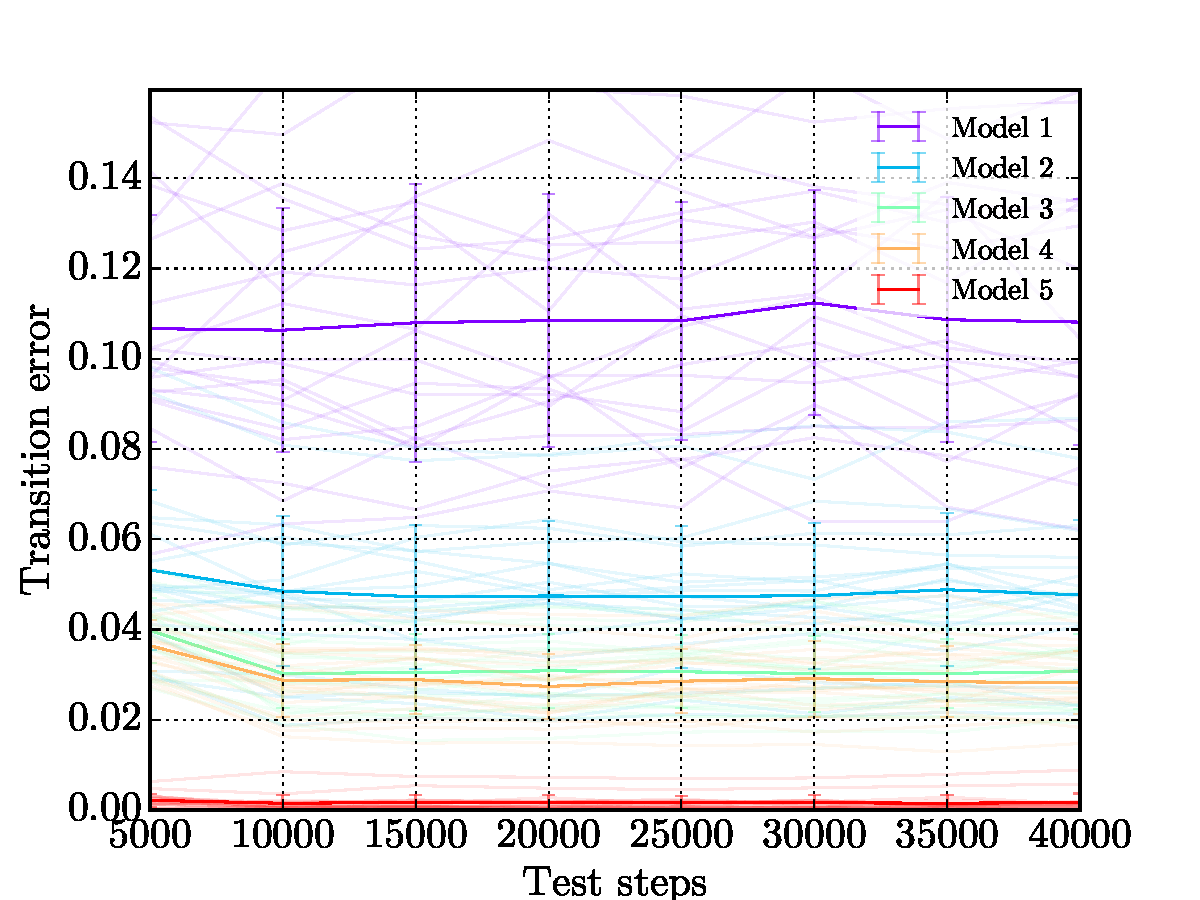
\includegraphics[width=\textwidth]{appendix/etaip_test_traces_distances_hugehip}
        \caption{$\eta_\IP = 0.002$}
        \label{fig:eta-huge}
    \end{subfigure}
    \begin{subfigure}{0.48\textwidth}
    	\centering
        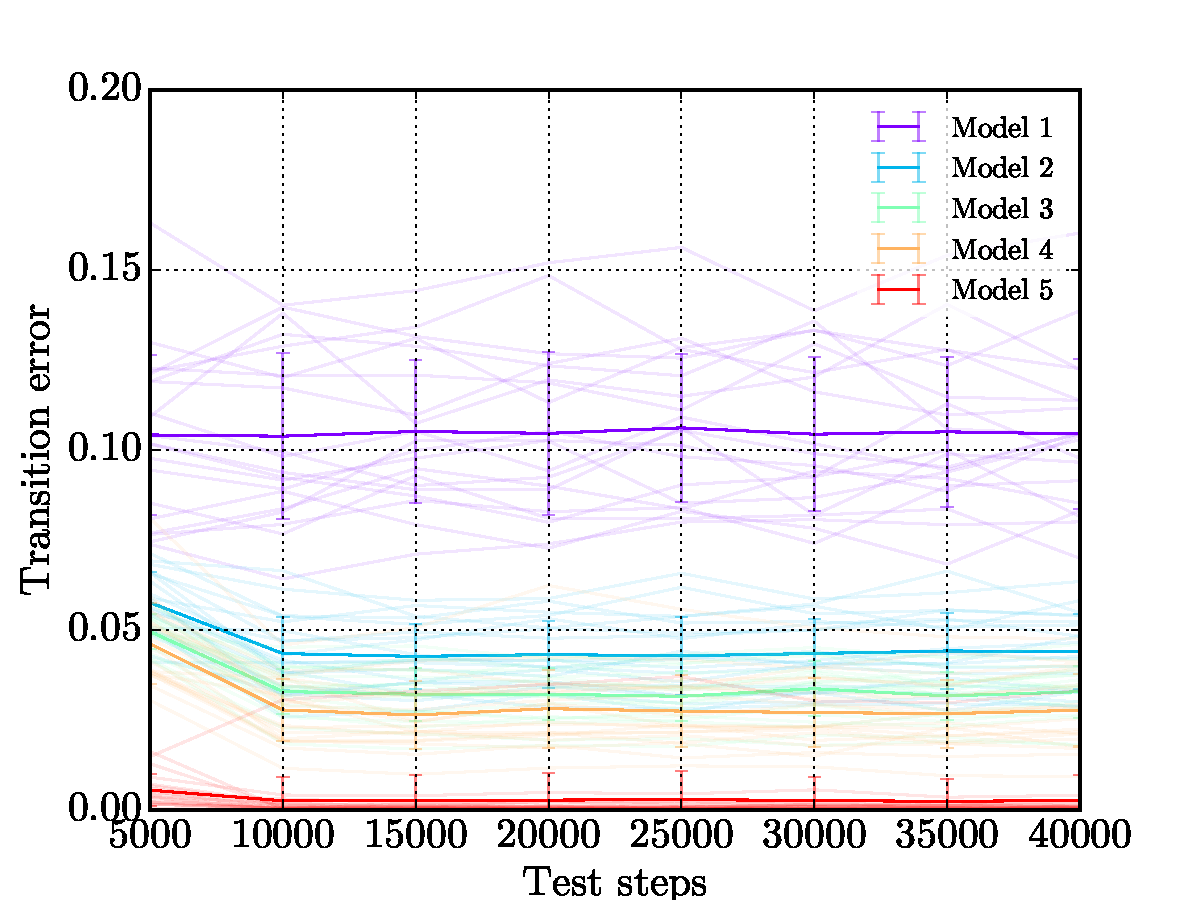
\includegraphics[width=\textwidth]{appendix/etaip_test_traces_distances}
        \caption{$\eta_\IP = 0.001$ (default)}
        \label{fig:eta-norm}
    \end{subfigure}
    \caption[Influence of the IP learning rate]{Influence of the \acs{ip} learning rate $\eta_\IP$ on the burn-in time in the beginning of the testing phase.}
    \label{fig:eta-ip}
\end{figure}

\clearpage

\subsection{Network connectivity}
\label{sec:appendix:connectivity}

As already mentioned at the end of results section \ref{sec:ip-hyp}, probably the connectivity could influence the performance, beside the \acl{ip}. The connectivity is defined by the number of connections of every neuron, which equals the number of weights with $w_{ij} > 0$ or --- under a biological perspective --- the number of synapses. Initially, every neuron is connected with $\rho = 0.1 \hat{=} 10\%$ of the other neurons. Since $N^E = 200$, every neuron has $\lambda^W = \rho \cdot N^E = 20$ synapses or weights greater zero. 

\begin{figure}[!b]
    \centering
    \begin{subfigure}{0.48\textwidth}
    	\centering
        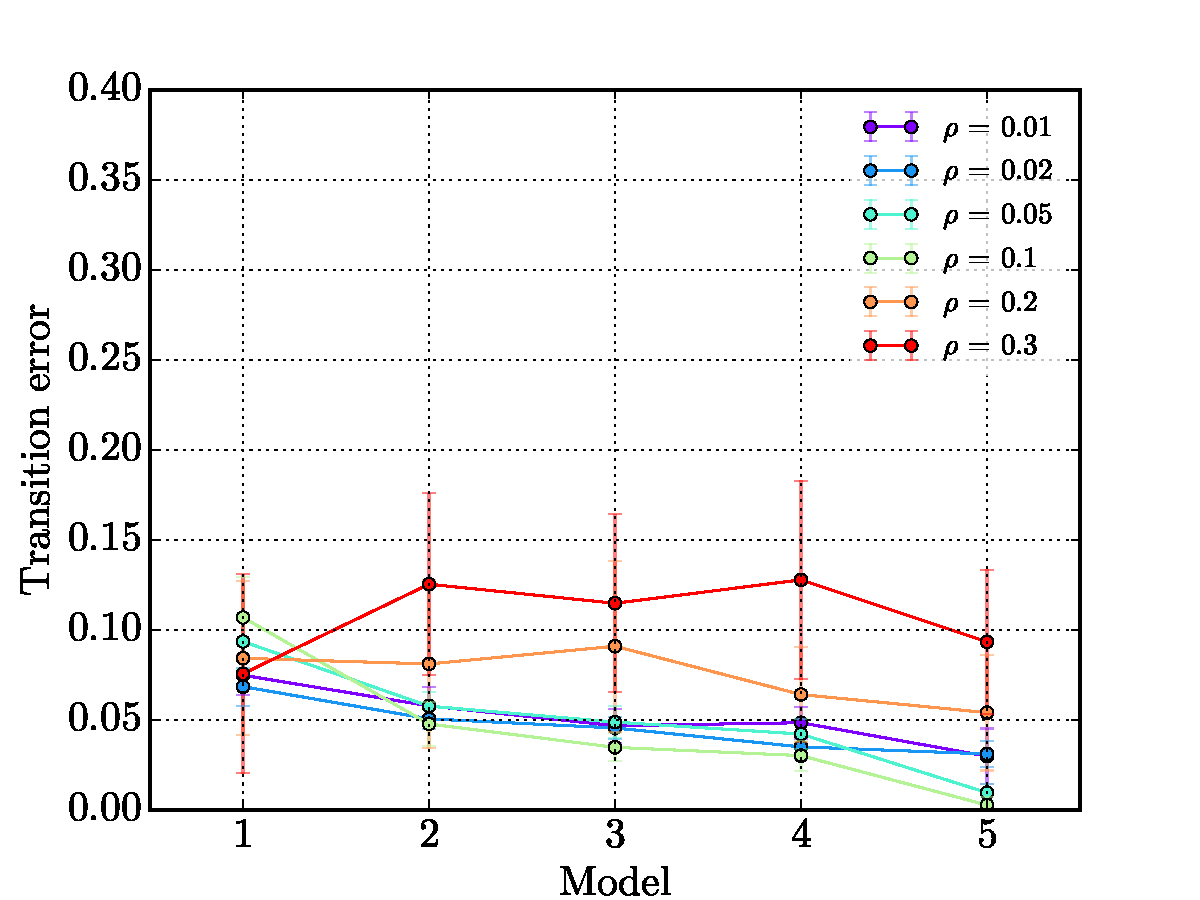
\includegraphics[width=\textwidth]{appendix/connectivity_plastic}
        \caption{Plastic reservoir ($T_\plastic = 50,000$)}
        \label{fig:connectivity-plastic}
    \end{subfigure}
    \hfill
    \begin{subfigure}{0.48\textwidth}
    	\centering
        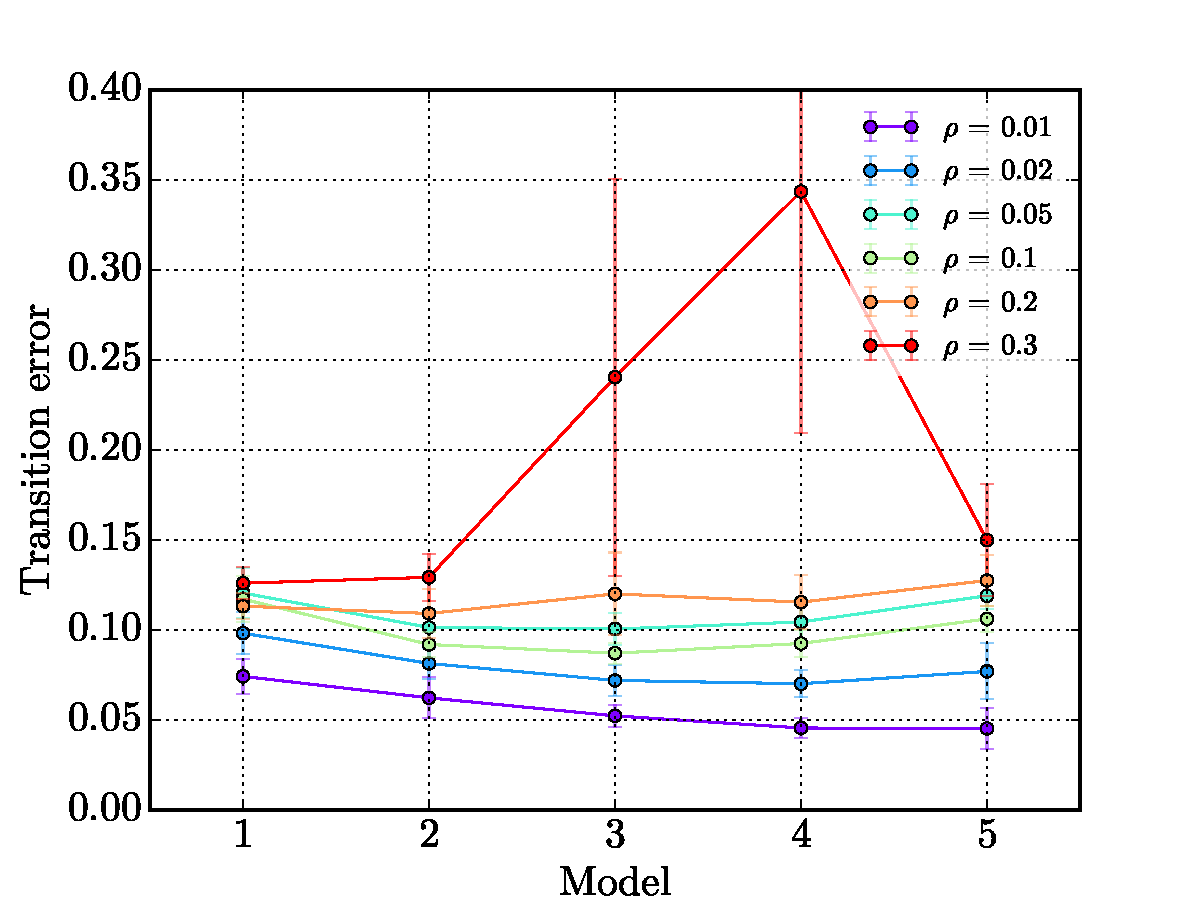
\includegraphics[width=\textwidth]{appendix/connectivity_static}
        \caption{Static reservoir ($T_\plastic = 0$)}
        \label{fig:connectivity-static}
    \end{subfigure}
    \caption[Variation of connectivity]{Variation of connectivity $\rho$. The left plot shows results for a plastic reservoir and the right plot for a static reservoir. For both holds that the more sparse the network is connected, the better the performance. Furthermore, the plastic reservoir outperforms the static reservoir network.}
    \label{fig:connectivity}
\end{figure}

\textcite{lazar2009sorn} showed in their appendix that the connectivity influences the performance of the network. In particular, they concluded that if the network is too dense, the activity `explodes'. To replicate the results in a context of Markov chain sampled input, model series II from figure \ref{fig:mc2-models} was divided into $5$ models. The results for different values of $\rho$ are shown in figure \ref{fig:connectivity}. On the left side the results for a \acs{sorn} with $T_\plastic = 50,000$ steps show that the performance is similar for $\rho \le 0.1$ and increases for $\rho > 0.1$. On the left side, a static reservoir is shown with $T_\plastic = 0$ steps. In that case, performance is increasing if $\rho$ increases. For $T_\plastic = 50,000$ steps and $\rho= 0.3$ the static reservoir network has very low performance in representing model $3$ and model $4$. \textcite{lazar2009sorn} suggested that this behavior is due to seizure-like bursts in the network, due to the high connectivity. Comparing both plots, a sparse connectivity increases the performance for both networks, plastic and static. Furthermore, the plastic network outperforms the static reservoir network. Both findings are in line with previous findings from \textcite{lazar2009sorn}.


